%%% TEMPLATE-INFO
%% Copied from     	: https://github.com/RUB-NDS/thesis_layout
%% Original AUTHOR	: vladislav.mladenov@rub.de
%%% Send him love, money or donuts if you find this template useful
%% Some texts/parts also stolen from the template of the Codes and Cryptography group at UPB

\RequirePackage{fix-cm,cmap}

\documentclass[
fontsize=11pt,
paper=a4,
abstract=true,
numbers=noenddot,
listof=totoc,
bibliography=totoc,
open=right,
cleardoublepage=plain,
parskip=half+, % comment this out if you do not want an empty half line between paragraphs, but please read the KomaScript Guide and search for parskip (around page 82): ftp://ftp.dante.de/pub/tex/macros/latex/contrib/koma-script/scrguide.pdf
BCOR=1cm, % Bindekorrektur: Change this accordingly, also read the KomaScript Guide! Make sure you read the guide.
]{scrreprt}

% ******************************************************************************
% ****************************** Custom Margin *********************************

% Add `custommargin' in the document class options to use this section
% Set {innerside margin / outerside margin / topmargin / bottom margin}  and
% other page dimensions
\ifsetCustomMargin
  \RequirePackage[left=37mm,right=30mm,top=35mm,bottom=30mm]{geometry}
  \setFancyHdr % To apply fancy header after geometry package is loaded
\fi

% Add spaces between paragraphs
%\setlength{\parskip}{0.5em}
% Ragged bottom avoids extra whitespaces between paragraphs
\raggedbottom
% To remove the excess top spacing for enumeration, list and description
%\usepackage{enumitem}
%\setlist[enumerate,itemize,description]{topsep=0em}

% *****************************************************************************
% ******************* Fonts (like different typewriter fonts etc.)*************

% Add `customfont' in the document class option to use this section

\ifsetCustomFont
  % Set your custom font here and use `customfont' in options. Leave empty to
  % load computer modern font (default LaTeX font).
  %\RequirePackage{helvet}

  % For use with XeLaTeX
  %  \setmainfont[
  %    Path              = ./libertine/opentype/,
  %    Extension         = .otf,
  %    UprightFont = LinLibertine_R,
  %    BoldFont = LinLibertine_RZ, % Linux Libertine O Regular Semibold
  %    ItalicFont = LinLibertine_RI,
  %    BoldItalicFont = LinLibertine_RZI, % Linux Libertine O Regular Semibold Italic
  %  ]
  %  {libertine}
  %  % load font from system font
  %  \newfontfamily\libertinesystemfont{Linux Libertine O}
\fi

% *****************************************************************************
% **************************** Custom Packages ********************************

% ************************* Algorithms and Pseudocode **************************

%\usepackage{algpseudocode}


% ********************Captions and Hyperreferencing / URL **********************

% Captions: This makes captions of figures use a boldfaced small font.
%\RequirePackage[small,bf]{caption}

\RequirePackage[labelsep=space,tableposition=top]{caption}
\renewcommand{\figurename}{Fig.} %to support older versions of captions.sty


% *************************** Graphics and figures *****************************

%\usepackage{rotating}
%\usepackage{wrapfig}

% Uncomment the following two lines to force Latex to place the figure.
% Use [H] when including graphics. Note 'H' instead of 'h'
%\usepackage{float}
%\restylefloat{figure}

% Subcaption package is also available in the sty folder you can use that by
% uncommenting the following line
% This is for people stuck with older versions of texlive
%\usepackage{sty/caption/subcaption}
\usepackage{subcaption}
% ********************************** Tables ************************************
\usepackage{booktabs} % For professional looking tables
\usepackage{multirow}

%\usepackage{multicol}
%\usepackage{longtable}
%\usepackage{tabularx}

% *********************************** SI Units *********************************
\usepackage{siunitx} % use this package module for SI units
\usepackage{tikz}

\newcommand*{\priority}[1]{\begin{tikzpicture}[scale=0.13]%
  \draw (0,0) circle (1);
  \fill[fill opacity=1.0,fill=red] (0,0) -- (90:1) arc (90:90-#1*3.6:1) -- cycle;
  \end{tikzpicture}}

\usepackage{hyperref}

\hypersetup{
    colorlinks=false,
    linkcolor=black,
    filecolor=magenta,
    pdfpagemode=FullScreen,
}
\urlstyle{same}
% ******************************* Line Spacing *********************************

% Choose linespacing as appropriate. Default is one-half line spacing as per the
% University guidelines

% \doublespacing
% \onehalfspacing
% \singlespacing


% ************************ Formatting / Footnote *******************************

% Don't break enumeration (etc.) across pages in an ugly manner (default 10000)
%\clubpenalty=500
%\widowpenalty=500

% \usepackage[perpage]{footmisc} %Range of footnote options


% *****************************************************************************
% *************************** Bibliography  and References ********************

%\usepackage{cleveref} %Referencing without need to explicitly state fig /table

% Add `custombib' in the document class option to use this section
\ifuseCustomBib
   \RequirePackage[square, sort, numbers, authoryear]{natbib} % CustomBib

% If you would like to use biblatex for your reference management, as opposed to the default `natbibpackage` pass the option `custombib` in the document class. Comment out the previous line to make sure you don't load the natbib package. Uncomment the following lines and specify the location of references.bib file

%\RequirePackage[backend=biber, style=numeric-comp, citestyle=numeric, sorting=nty, natbib=true]{biblatex}
%\addbibresource{References/references} %Location of references.bib only for biblatex, Do not omit the .bib extension from the filename.

\fi

% changes the default name `Bibliography` -> `References'
\renewcommand{\bibname}{References}


% ******************************************************************************
% ************************* User Defined Commands ******************************
% ******************************************************************************

% *********** To change the name of Table of Contents / LOF and LOT ************

%\renewcommand{\contentsname}{My Table of Contents}
%\renewcommand{\listfigurename}{My List of Figures}
%\renewcommand{\listtablename}{My List of Tables}


% ********************** TOC depth and numbering depth *************************

\setcounter{secnumdepth}{2}
\setcounter{tocdepth}{2}


% ******************************* Nomenclature *********************************

% To change the name of the Nomenclature section, uncomment the following line

%\renewcommand{\nomname}{Symbols}


% ********************************* Appendix ***********************************

% The default value of both \appendixtocname and \appendixpagename is `Appendices'. These names can all be changed via:

%\renewcommand{\appendixtocname}{List of appendices}
%\renewcommand{\appendixname}{Appndx}

% *********************** Configure Draft Mode **********************************

% Uncomment to disable figures in `draft'
%\setkeys{Gin}{draft=true}  % set draft to false to enable figures in `draft'

% These options are active only during the draft mode
% Default text is "Draft"
%\SetDraftText{DRAFT}

% Default Watermark location is top. Location (top/bottom)
%\SetDraftWMPosition{bottom}

% Draft Version - default is v1.0
%\SetDraftVersion{v1.1}

% Draft Text grayscale value (should be between 0-black and 1-white)
% Default value is 0.75
%\SetDraftGrayScale{0.8}


% ******************************** Todo Notes **********************************
%% Uncomment the following lines to have todonotes.

\ifsetDraft
	\usepackage[colorinlistoftodos]{todonotes}
	\newcommand{\mynote}[1]{\todo[author=kks32,size=\small,inline,color=green!40]{#1}}
\else
	\newcommand{\mynote}[1]{}
	\newcommand{\listoftodos}{}
\fi

% Example todo: \mynote{Hey! I have a note}

% ******************************** Highlighting Changes **********************************
%% Uncomment the following lines to be able to highlight text/modifications.
%\ifsetDraft
%  \usepackage{color, soul}
%  \newcommand{\hlc}[2][yellow]{{\sethlcolor{#1} \hl{#2}}}
%  \newcommand{\hlfix}[2]{\texthl{#1}\todo{#2}}
%\else
%  \newcommand{\hlc}[2]{}
%  \newcommand{\hlfix}[2]{}
%\fi

% Example highlight 1: \hlc{Text to be highlighted}
% Example highlight 2: \hlc[green]{Text to be highlighted in green colour}
% Example highlight 3: \hlfix{Original Text}{Fixed Text}

% *****************************************************************************
% ******************* Better enumeration my MB*************
\usepackage{enumitem}
\usepackage{url}

% ********************************* Acronyms ****************************************
\usepackage{acro}
\DeclareAcronym{ui}{
  short=UI,
  long=User Interface,
}

\DeclareAcronym{mbse}{
  short=MBSE,
  long=Model-Based Software Engineering,
}

\DeclareAcronym{html}{
  short=HTML,
  long=Hypertext Markup Language,
}

\DeclareAcronym{ucd}{
  short=UCD,
  long=User-Centered Design,
}

\DeclareAcronym{it}{
  short=IT,
  long=Information Technology,
}

\DeclareAcronym{lcdp}{ 
  short=LCDP,
  long=Low-Code Development Platform,
}

\DeclareAcronym{ncdp}{
  short=NCDP,
  long=No-Code Development Platform,
}

\DeclareAcronym{db}{
  short=DB,
  long=Database,
}

\DeclareAcronym{dbms}{
  short=DBMS,
  long=Database Management System,
}

\DeclareAcronym{ds}{
  short=DS,
  long=Data Structure,
}

\DeclareAcronym{dml}{
  short=DML,
  long=Data Modeling Language,
}

\DeclareAcronym{dsl}{
  short=DSL,
  long=Domain Specific Language,
}

\DeclareAcronym{csv}{
  short=CSV,
  long=Comma Separated Value,
}

\DeclareAcronym{api}{
  short=API,
  long=Application Programming Interfaces,
}

\DeclareAcronym{rest}{
  short=REST,
  long=Representational State Transfer,
}

\DeclareAcronym{gui}{
  short=GUI,
  long=Graphical User Interface,
}

\DeclareAcronym{mvc}{
  short=MVC,
  long=Model-View-Controller,
}

\DeclareAcronym{uat}{
  short=UAT,
  long=User Acceptance testing,
}

\DeclareAcronym{mqtt}{
  short=MQTT,
  long=Message Queue Telemetry Transport,
}

\DeclareAcronym{mdse}{
  short=MDSE,
  long=Model Driven Software Engineering,
}

\DeclareAcronym{mof}{
  short=MOF,
  long=Model Object Facility,
}

\DeclareAcronym{omg}{
  short=OMG,
  long=Object Management Group,
}

\DeclareAcronym{uml}{
  short=UML,
  long=Unified Modeling Language,
}

\DeclareAcronym{se}{
  short=SE,
  long=Software Engineering,
}

\DeclareAcronym{mdd}{
  short=MDD,
  long=Model Driven Development,
}

\DeclareAcronym{ce}{
  short=CE,
  long=Continuous Experimentation,
}

\DeclareAcronym{ux}{
  short=UX,
  long=User Experience,
}

\DeclareAcronym{mvp}{
  short=MVP,
  long=Minimum Viable Product,
}

\DeclareAcronym{dr}{
  short=DR,
  long=Design Requirements,
}

\DeclareAcronym{dp}{
  short=DP,
  long=Design Principles,
}

\DeclareAcronym{df}{
  short=DF,
  long=Design Features,
}

\DeclareAcronym{desy}{
  short=DeSy,
  long=Design System,
}

\DeclareAcronym{pc}{
  short=PC,
  long=Personal Computer,
}

\DeclareAcronym{dsr}{
  short=DSR,
  long=Design Science Research,
}

\DeclareAcronym{crud}{
  short=CRUD,
  long=Create Read Update Delete
}

\DeclareAcronym{poc}{
  short=POC,
  long=Proof-Of-Concept
}

\DeclareAcronym{soa}{
  short=SOAT,
  long=State Of The Art
}

\DeclareAcronym{sa}{
  short=SA,
  long=Software Approach
}

\DeclareAcronym{ra}{
  short=RA,
  long=Related Approach
}

\DeclareAcronym{cli}{
  short=CLI,
  long=Command-Line Interface
}

\DeclareAcronym{sus}{
  short=SUS,
  long=System Usability Score
}

%% here your document starts
\begin{document}

%% switch to roman paginating for the acknowledgements, table of contents etc.
\pagenumbering{roman} % uncomment this if you like it

%% title page --- made out of expressions defined above
% Hintergrund-Makro
\newcommand\BackgroundPic{
\put(0,0){
\parbox[b][\paperheight]{\paperwidth}{%
\vfill
\centering

\includegraphics[width=\paperwidth,height=\paperheight]{images/front.png}%
\vfill
}}}

\AddToShipoutPicture*{\BackgroundPic}
\begin{titlepage}
\makeatletter

\enlargethispage{3cm}

\begin{minipage}[b]{1\linewidth}
	\sffamily
	
\includegraphics[scale=0.5]{images/upb_logo.pdf}
  	\vspace*{8cm}
  	
	\textbf{\LARGE {\@title}}\\
  
	\Large{\@author}\\
	
% 	\vspace*{35mm}
	\vspace{4cm}
	\normalsize{
	Exposé/Proposal\@~~--~~\@date\@.\\
	Our Group Name.\\}
	\newline
	\normalsize{
	\begin{tabular}{@{}ll@{}}
	Supervisor: 	& Dr. Enes Yigitbas\\
					& Prof. Dr. Gregor Engels\\
	\end{tabular}
	}
\end{minipage}


\makeatother
\end{titlepage}
\ClearShipoutPicture


\pagenumbering{arabic} %switches to arabic numbers for the rest of the text
\setcounter{page}{1}
\tableofcontents

\chapter{Introduction} \label{chap:intro}
This chapter explains the problems faced by the companies during Software development (see section \ref{intro:section:problems}), our Research approach (see section \ref{intro:section:research}), and finally, our solution approach (see section \ref{intro:section:solution}).

\section{Motivation}
Over the last decade, Software development had a tremendous impact with increasing customer demand and requirements \cite{article:swdemand:ahmed}. 
The product designers responsible for designing various product variants are unsure which variant would be most liked by the customers.
Similarly, increasing product complexity and ambiguity significantly impact software development. 
So, the developers have come up with different techniques to meet this requirement criteria.
Early user feedback from potential customers in the industry is crucial for creating successful software products because of the growing market uncertainties, and consumers' desire to receive integrated solutions to their issues rather than unique software developments \cite{misc:businessmodels:teece}.
With the increasing complexity of products, it becomes challenging to determine user requirements making it more difficult for developers to assess their opinions.
As a result, the developers of these products are biased toward some requirements and can ignore what the user wants. 
We must detect the user's needs and requirements to reduce these risks early. 
Giving users a ``partially functioning'' system is the most excellent method to determine their requirements and suggestions \cite{journal:prototyping:davis}.
This ensures that the developers with high uncertainties in the early product development can validate by testing the underlying assumptions \cite{misc:lean:steve}.
Developers can use this feedback to validate the most critical assumptions about the software product. 
This validation can be used to decide whether to add, remove or update a feature \cite{article:experiments:lindgren}. 
This process of determining the best fit for the product through user feedback is called experimentation.
There has been an increase in interest in the types of experimentation that can take place in product development. 
Software products have shown the benefits of conducting experiments in many use cases with incremental product improvement \cite{article:controlled:experiements}.
In Experimentation, the product designers design different UI variants (e.g., buttons with different colors), and the developer integrates these variants and assigns them to a distinct group of users. 
As per some evaluation criteria, the variant with better results is deployed for the entire set of users.
So, an experiment can be valuable when it improves the software products.
Hence, for experiments to be successful, they should offer one or more solutions that will benefit users.

\section{Problem Statement}
\label{intro:section:problems}
This section explains the current problems faced by developers during software development. 
We define three problems and determine the research and the solution approach for the same.

\paragraph{Problem 1:} Product designers create many UI prototypes, and the developers implement them.
To determine the best variant, the developers create experiments with the users. 
This concrete implementation of designs uses a lot of resources and time for the developers.
Therefore, the product designers need to be integrated into the development process so that they would be able to create experiments independent of the developers.

% \paragraph{Problem 2:} (Use design principles)

\paragraph{Problem 2:} When the product designers develop the prototypes, testing them with many users is difficult as the product is still not developed.
Therefore, it is not easy to conclude a ``winner'' variant with a small amount of data as it is statistically difficult to prove one of the variants outperforms the others \cite{article:usability:smalldata}.
Therefore, it is necessary to develop an idea that the designers can use to determine the best prototype or variant with a small group of users.

\paragraph{Problem 3:} Most often, the software application collects data from the experiments. 
Some data is used in Qualitative analysis, while others are in Quantitative analysis.
Many companies fail to reap the benefits of using both Qualitative and Quantitative analysis.
Similarly, not all the data is used in the analysis phase reducing the software applications to improve based on customer feedback \cite{article:datadrive:brian}.
Therefore, finding a solution that combines qualitative and quantitative data analysis is necessary.

\section{Research Approach}
\label{intro:section:research}
\begin{figure}[ht]
    \centering
    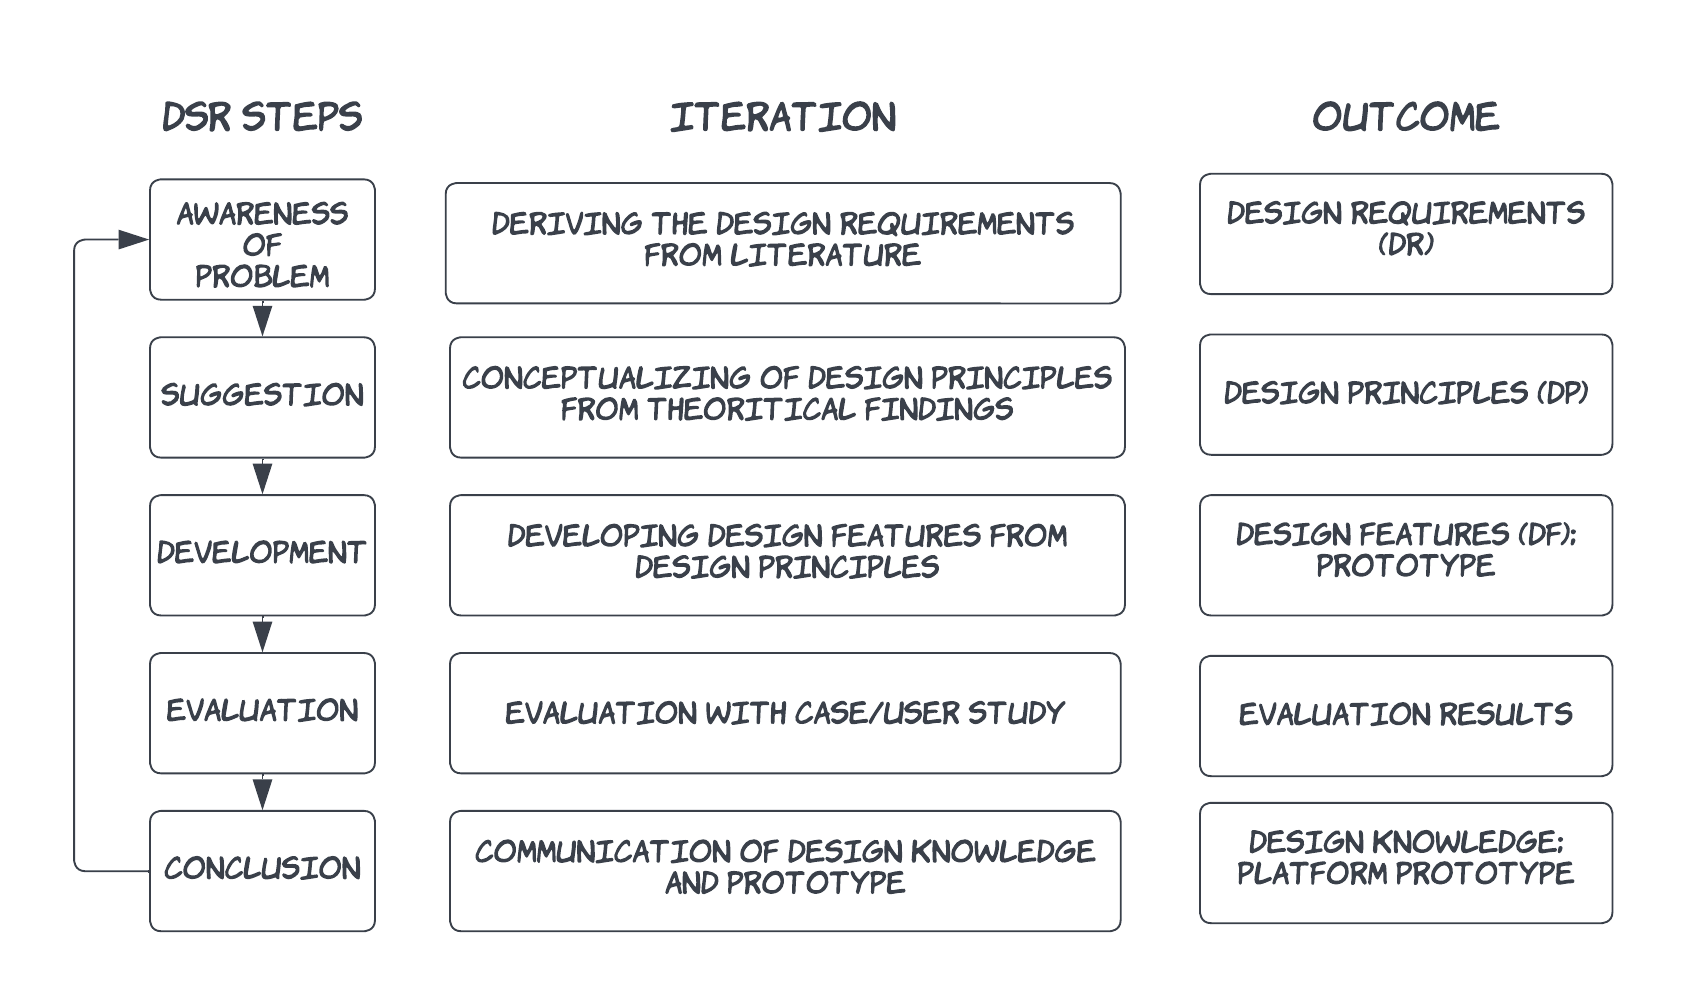
\includegraphics[scale=0.2]{images/solution-ideas/DSRcycle.png}
    \caption{Design Science Research Cycle \cite{paper:designprinciple:vk}}
    \label{intro:fig:dps}
\end{figure}
This section identifies the Research Question (RQ) and defines an approach to answer the question.
\paragraph{RQ:}How to develop a platform suitable for product designers to conduct experiments on UI prototypes, increasing its usability and, at the same time, independent of developers?

% The process of creating experiments and testing their variants is usually not systematically arranged, creating anomalies, and leading to unsuccessful experiments.
To answer this question, we will conduct a design science research (DSR) study to obtain some Design Principles (DPs) defined for the whole process of experimentation \cite{paper:designprinciple:vk}. 
Here, DPs capture and codify that knowledge by focussing on the implementer, the aim, the user, the context, the mechanism, the enactors, and the rationale \cite{paper:designprinciple:gregor}. 
The DPs explain the design information that develops features for software applications.
We propose to use the variation of the cycle of Kuechler and Vaishnavi \cite{paper:designprinciple:vk} consisting of five iteratively conducted steps (see figure \ref{intro:fig:dps}). 
First, we identify the 
\texttt{(1) Awareness of the Problem} and provide a
\texttt{(2) Suggestion of a possible solution}. Next, we work on the 
\texttt{(3) Development of the software artifact} and conduct an 
\texttt{(4) Evaluation} of it. Based on the evaluation results, we provide 
\texttt{(5) Conclusions} \cite{misc:crowdsourcing:sg}.
From each step of the DSR, we have an iteration cycle and an outcome (e.g., Awareness of the Problem leads to finding Design Requirements, Design Principles (DPs) can be found from the Suggestion of the solution, Development of the software artifact leads to finding the Design Features and the Prototype, etc.) as shown in figure \ref{intro:fig:dps}.
Therefore through the use of DSR, a group of issues is resolved by concentrating on a single issue and abstracting the consequences of the resolution.


\section{Solution Approach}
\label{intro:section:solution}
To solve the problems mentioned above, the designers should be able to create UI prototypes and experiments on their own on a set of users.
Since we do not have a large set of users for testing the prototypes, we use supervised task-based usability testing \cite{article:dataanalysis:supervisedtest}.
The fundamental principle of task-based usability testing is to have the users attempt to use the prototypes to do certain activities or tasks (e.g., Locate a movie M1) and get feedback (e.g., the time required for the task to be completed by the user).
We propose to use \texttt{Low-code} or \texttt{No-Code} approach to achieve this.
This approach helps to have a UI interface for the designers to understand, develop, and create experiments and tasks with the software prototypes \cite{paper:lowcode:khorram}.
So, the designers would be able to test the UI prototypes, assign them to the users, get feedback from the users and decide on the best prototype.
At the same time, the Low-code has become more accessible for Model-driven development.
Therefore, we plan to create models for the UI prototypes and have the feasibility for creating experiments and tasks. 
Because of using the models, it is easier to store the prototypes in the database and conduct experiments with the users. 

\begin{figure}[ht]
    \centering
    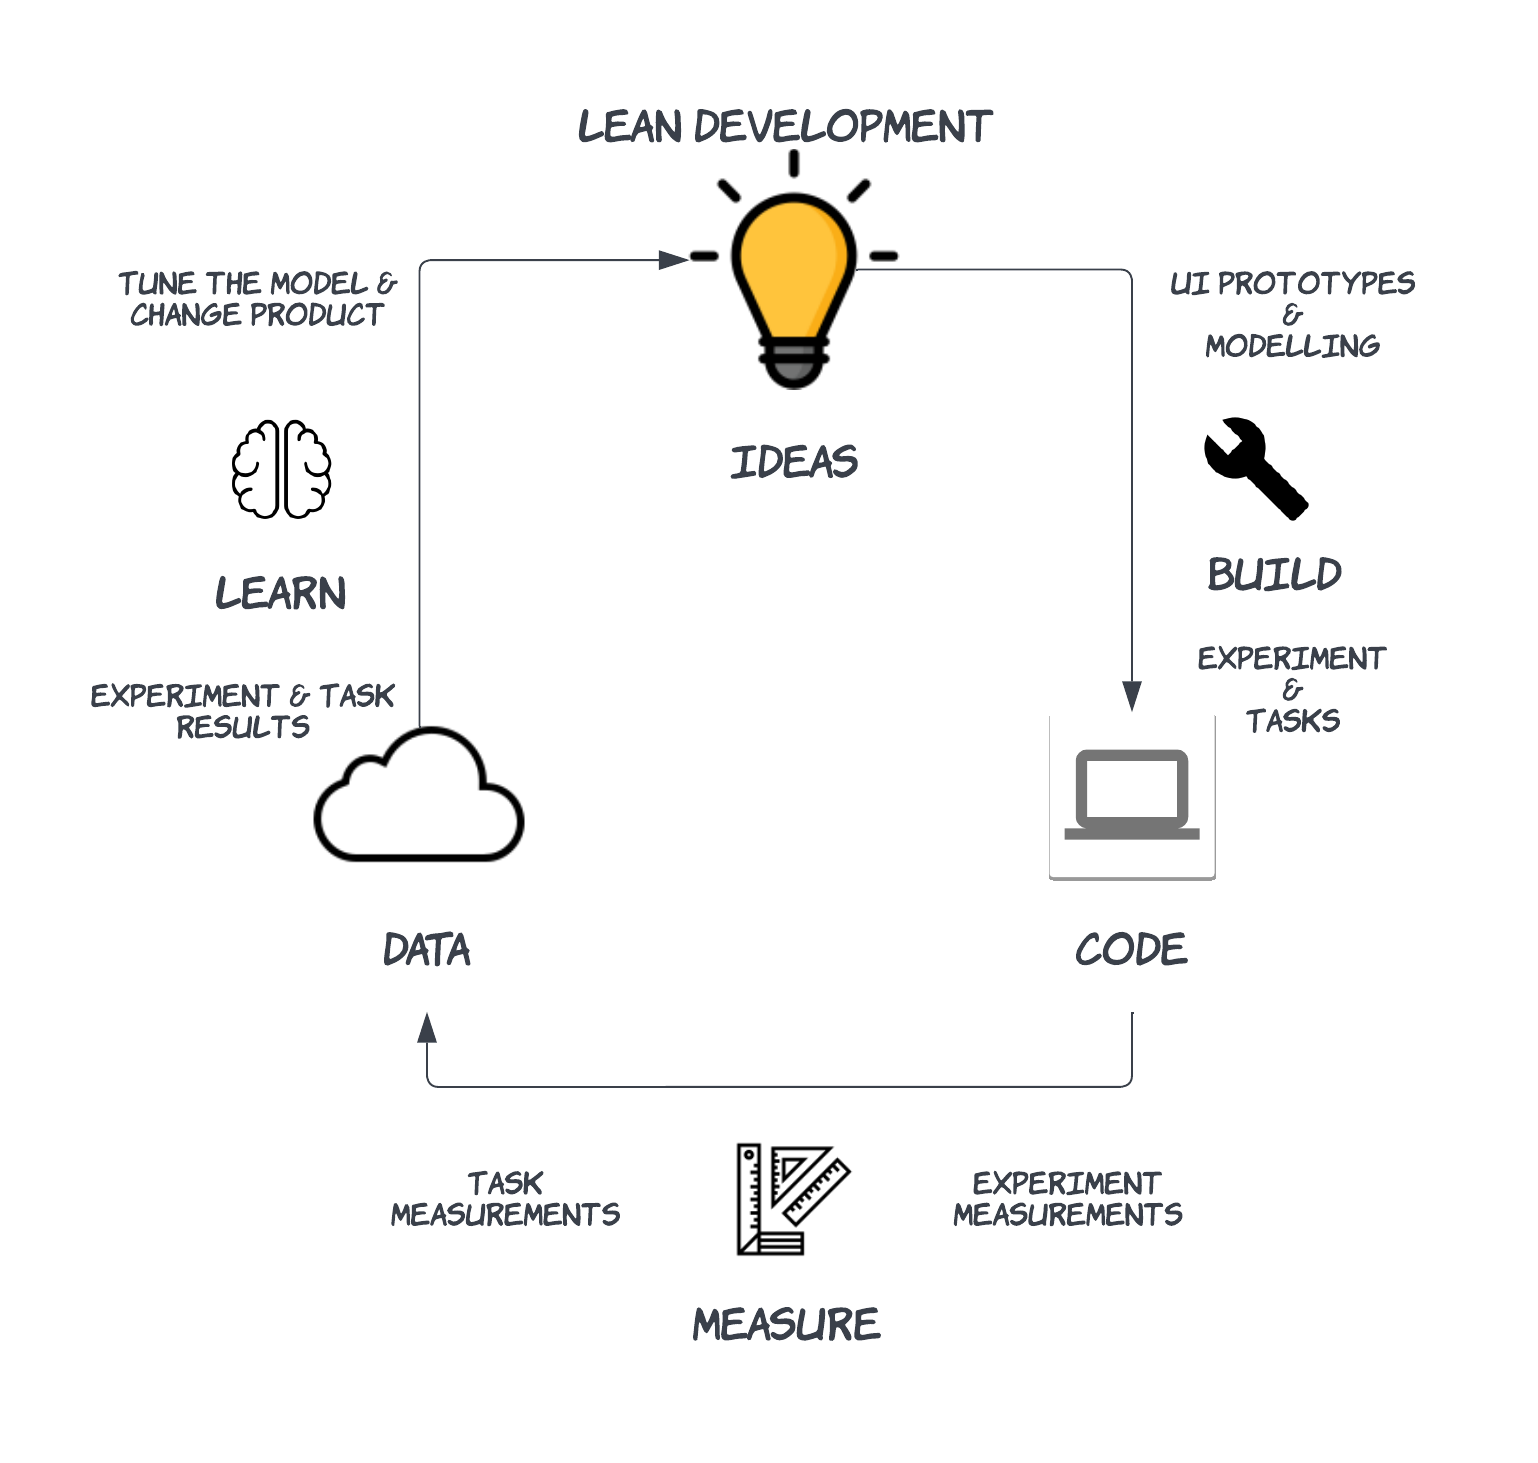
\includegraphics[scale=0.15]{images/solution-ideas/LEAN.png}
    \caption{LEAN Development technique}
    \label{intro:fig:lean}
\end{figure}

In our solution, we use the LEAN development technique (see figure \ref{intro:fig:lean}) for development as it is used to develop customers friendly products \cite{article:lean:hart}.
Using LEAN, the company creates a Minimum Viable Product (MVP) throughout development, tests it with potential customers, and leverages their input to make incremental changes.
While this technique can be used for every product, there are also approaches specific to software products.
LEAN development technique can be divided into a Build, Measure, and Learn cycle. 
In the \texttt{(1) Build} phase, we plan to create the \texttt{UI Prototypes}, \texttt{Models}, \texttt{Experiments}, and \texttt{Tasks} for the users.
In the \texttt{(2) Measure} phase, we plan to assign the Experiments and Tasks to the users and measure the \texttt{Task and the Experiment measurements} and perform some analysis on the data received. 
And finally, in the \texttt{(3) Learn} phase, we display the \texttt{Analyses results}, \texttt{Tune} our models to decide the better variant among the others, and \texttt{Modify} the prototype.
As per the figure \ref{intro:fig:lean}, we complete one cycle of iteration and start a new one with the updated prototype.
The solution approach is explained more in detail in Chapter \ref{chap:solutionideas}.

% To solve the first problem, the developers focus more on automating the software code rather than coding everything stated in the product requirements \cite{article:prototyping:hoffnagle}.
% This approach is formally known as a \texttt{Low-code} or \texttt{No-Code} approach.
% So, this approach helps to have a UI interface for the non-developers to understand and develop the software products \cite{paper:lowcode:khorram}.
% One approach to support the product owners in developing the variants is UI Prototyping. 
% UI prototyping creates new UI variants using predefined UI elements (e.g., Drag and drop the UI element Button into the screen).
% This helps product owners to be creative and innovative because it gives them visual feedback.
% So, if UI prototypes are developed in a low-code technique, they would be lightweight software that helps the product owner develop various prototypes and conduct experiments on the users.
% According to Cabot et al. \cite{paper:lowcode:cabot}, the low-code has become more accessible for Model-driven development. 
% Similarly, while creating prototyping, the software should have connections between the screens (e.g., clicking on a button should go to the next screen), and this logic can be achieved using Models.
% Models are used broadly in prototyping because a model represents or describes the aspects of the systems that cannot be described adequately in a system of interest \cite{paper:prototyping:luqi}.
% Moderately accurate models can be created using an iterative approach in software development by getting continuous feedback from the users.


% To solve the \texttt{second} problem, we use supervised task-based usability testing \cite{article:dataanalysis:supervisedtest}.
% The fundamental principle of usability testing is to have real users attempt to use the software application to do certain activities.
% Observing users interact with an interface is the most efficient way to determine what functions well and what doesn't.
% The users will undertake realistic actions, giving us qualitative insights into the problems that users are experiencing and enhancing the design with these insights \cite{misc:usability:tasks}.
% These activities can be the tasks or scenarios (e.g., Locate a movie M1) for the users to complete and analyze (e.g., the time/clicks required to locate the Movie M1).

% To solve the \texttt{third} problem, the models should use data to measure the experiments' success for improvement. This process is called a Data-driven development approach. 
% This approach uses meaningful, actionable consumer feedback regarding the effects of the product experiments by using the \texttt{Qualitative and Quantitative} data analysis.
% Using a combination of qualitative and quantitative data can improve an evaluation by ensuring that the strengths of another balance the limitations of one type of data confirming that the knowledge is enhanced by integrating different techniques.




% In our solution, we use the LEAN development technique (see figure \ref{intro:fig:lean}) for development as it is used to develop customers friendly products \cite{article:lean:hart}.
% Using LEAN, the company creates a Minimum Viable Product (MVP) throughout development, tests it with potential customers, and leverages their input to make incremental changes.
% While this technique can be used for every product, there are also approaches specific to software products.
% LEAN development technique can be divided into a Build, Measure, and Learn cycle. 
% In the \texttt{(1) Build} phase, we plan to create the \texttt{UI Prototypes}, \texttt{Models}, \texttt{Experiments}, and \texttt{Tasks} for the users.
% In the \texttt{(2) Measure} phase, we plan to assign the Experiments and Tasks to the users and measure the \texttt{Task and the Experiment measurements} and perform some analysis on the data received. 
% And finally, in the \texttt{(3) Learn} phase, we display the \texttt{Analyses results}, \texttt{Tune} our models to decide the better variant among the others, and \texttt{Modify} the prototype.
% As per the figure \ref{intro:fig:lean}, we complete one cycle and start a new iteration.
% The solution approach is explained more in detail in Chapter \ref{chap:solutionideas}.
\chapter{Related Work} \label{chap:csr}

Explain what the current state of the research is and summarize related work. 
For example, you could write about: 
\begin{itemize}
	\item Figma\footnote{https://www.figma.com/}
	\item Others\footnote{https://webflow.com/blog/prototyping-tools} 	
	\item \dots
\end{itemize}

Note: \emph{This template is just an example.} You can of course combine Sections~\ref{chap:intro} and~\ref{chap:csr} into one section or use a different structure.
% \chapter{Goals of this Thesis} \label{chap:goals}

Give a short description of your thesis goals:

\begin{itemize}
	\item What is the problem with existing solutions or existing attacks? (i.e. with the stuff you explained in the previous section)
	\item What is the goal of the thesis in a nutshell? What problem can you solve? What algorithm/attack can you improve? Can you improve the solution as suggested by
	\item Explain how your evaluation will look like. Describe your test environment. Are you going to analyze local open source implementations and their potential vulnerabilities to your attacks? Are you going to perform systematic large-scale scanning of real devices on the Internet?\footnote{\textbf{Always} consult your supervisor if you want to perform large-scale scanning or real systems.}
	\item Provide optional goals.
\end{itemize}
\chapter{Solution Idea} \label{chap:solutionideas}

This section presents our plan for obtaining the objectives discussed in section \ref{chap:intro}. 
In our approach, we propose a Model-based approach using the LEAN development process. 
As mentioned earlier, LEAN contains three phases Build, Measure, and Learn.
In the \texttt{Build} phase, we plan to create the \texttt{(1) Visualization of Prototypes}, and \texttt{(2) Model} these prototypes for Experiments and Tasks.
In the \texttt{Measure} phase, we plan to \texttt{(3) Assign these prototypes to the users} and measure the \texttt{(4) Experiment and the Task measurements}.
Finally, in the \texttt{Learn} phase, we would analyze the results performing \texttt{(5) Different analyses}, and \texttt{(6) Improve our Prototype} from the analyses feedback.  

Consider an example of a \textbf{``A video streaming service''} called \texttt{VideoStreamer (VS)}.
We divide the different stakeholders of this company into developers (e.g., programmers, etc.) and non-developers (e.g., product designers).
% \begin{figure}
%     \centering
%     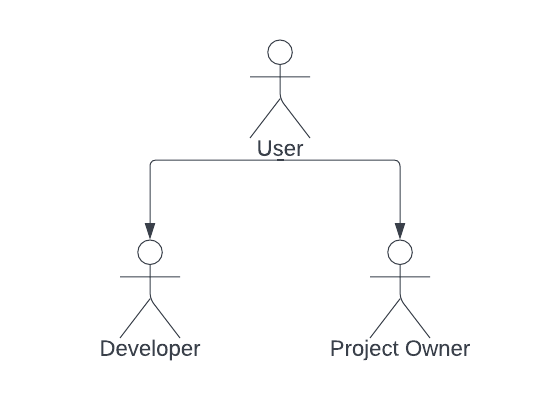
\includegraphics[scale=0.2]{images/solution-ideas/Stakeholder.png}
%     \caption{Different Stakeholders in the Company VS}
%     \label{solutionideas:fig:stakeholders}
%\end{figure}
Usually, the developers are responsible for developing various features required for the company. 
But, the problem is, in the beginning, knowing which design fits better for a UI is impossible. 
Therefore, we need to perform experiments on the UI using A/B testing.
So, the developers develop different variants for experimenting with the UI and get feedback from the non-developers.
This feedback process wastes a lot of time, so our solution is to give freedom to the product owners and reduce the gap between the product owners and the developers by allowing the product owners to create the UI using UI prototyping.

\section{Build}
In this step (as per figure \ref{intro:fig:lean}), we create ideas for the product and visualize the Prototypes (explained in section \ref{solutionideas:subsection:visualize}) and then Model them together for creating Experiments and Tasks for the users (explained in section \ref{solutionideas:subsection:modelling}).
We plan to implement the build step in a low-code or no-code technique for our solution because it needs negligible installation, setup, training, and implementation work.
The low-code or no-code technique enables software applications' rapid creation and deployment with little or no coding effort.

\subsection{Visualising the Prototypes}
\label{solutionideas:subsection:visualize}

We plan to create a system for non-developers to modify the UI elements in a canvas-like structure in an application using UI Prototyping.
For this, the non-developers first create a canvas screen and input the name for that screen.
As shown in figure \ref{solutionideas:fig:uiprototyping}, they can add UI elements like buttons, input buttons, select buttons, etc., on the canvas screen.
We propose to use angular\footnote{Angular: \url{https://angular.io/}} for developing the application.
Various UI elements are available for the drag and drop of the UI elements, as shown in figure \ref{solutionideas:fig:uiprototyping} (right side).

\begin{figure}[h]
    \centering
    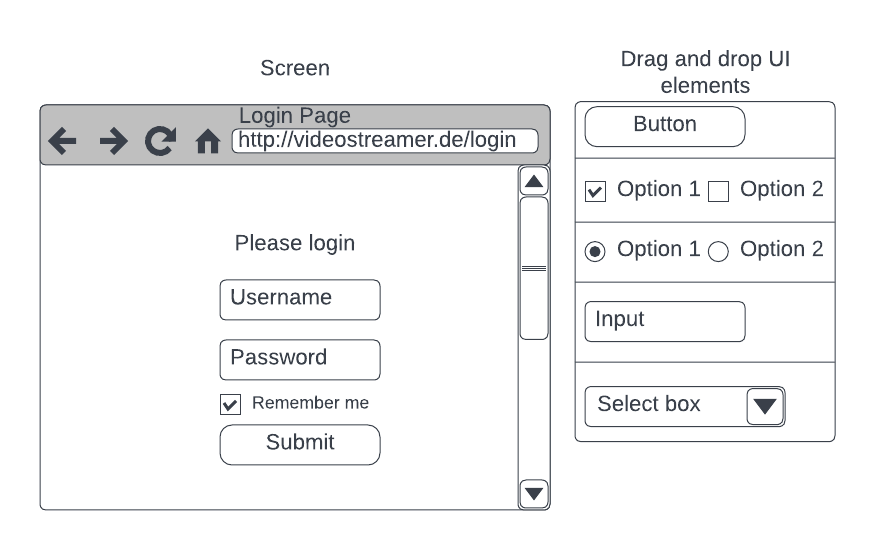
\includegraphics[scale=0.4]{images/solution-ideas/UIPrototyping.png}
    \caption{UI Prototyping using drag and drop of UI elements}
    \label{solutionideas:fig:uiprototyping}
\end{figure}

Once the non-developers finalize the UI screen, they can move to the next screen by some logic (e.g., clicking on a button to go to the next screen). 
This way, the non-developers can design the entire application, having a sequential flow (i.e., the user will register, go to the Login page, next to the Dashboard page, etc.), using the canvas screen, and adjust the UI elements.
At the same time, the non-developers can build the entire application quickly without any programming knowledge.

\subsection{Modelling the Prototypes}
\label{solutionideas:subsection:modelling}

In our application, we plan to convert the screens the non-developers develop into models. 
To do that, we need a modeling language that fits our requirements. As per figure \ref{solutionideas:fig:metamodel}, we first create the meta models, then build concrete models out of these to store the properties of the prototypes as attributes.
Therefore, we need concrete models for \texttt{Experiments}, \texttt{Tasks} and \texttt{Prototypes}.

\begin{figure}[bt]
	\centering
  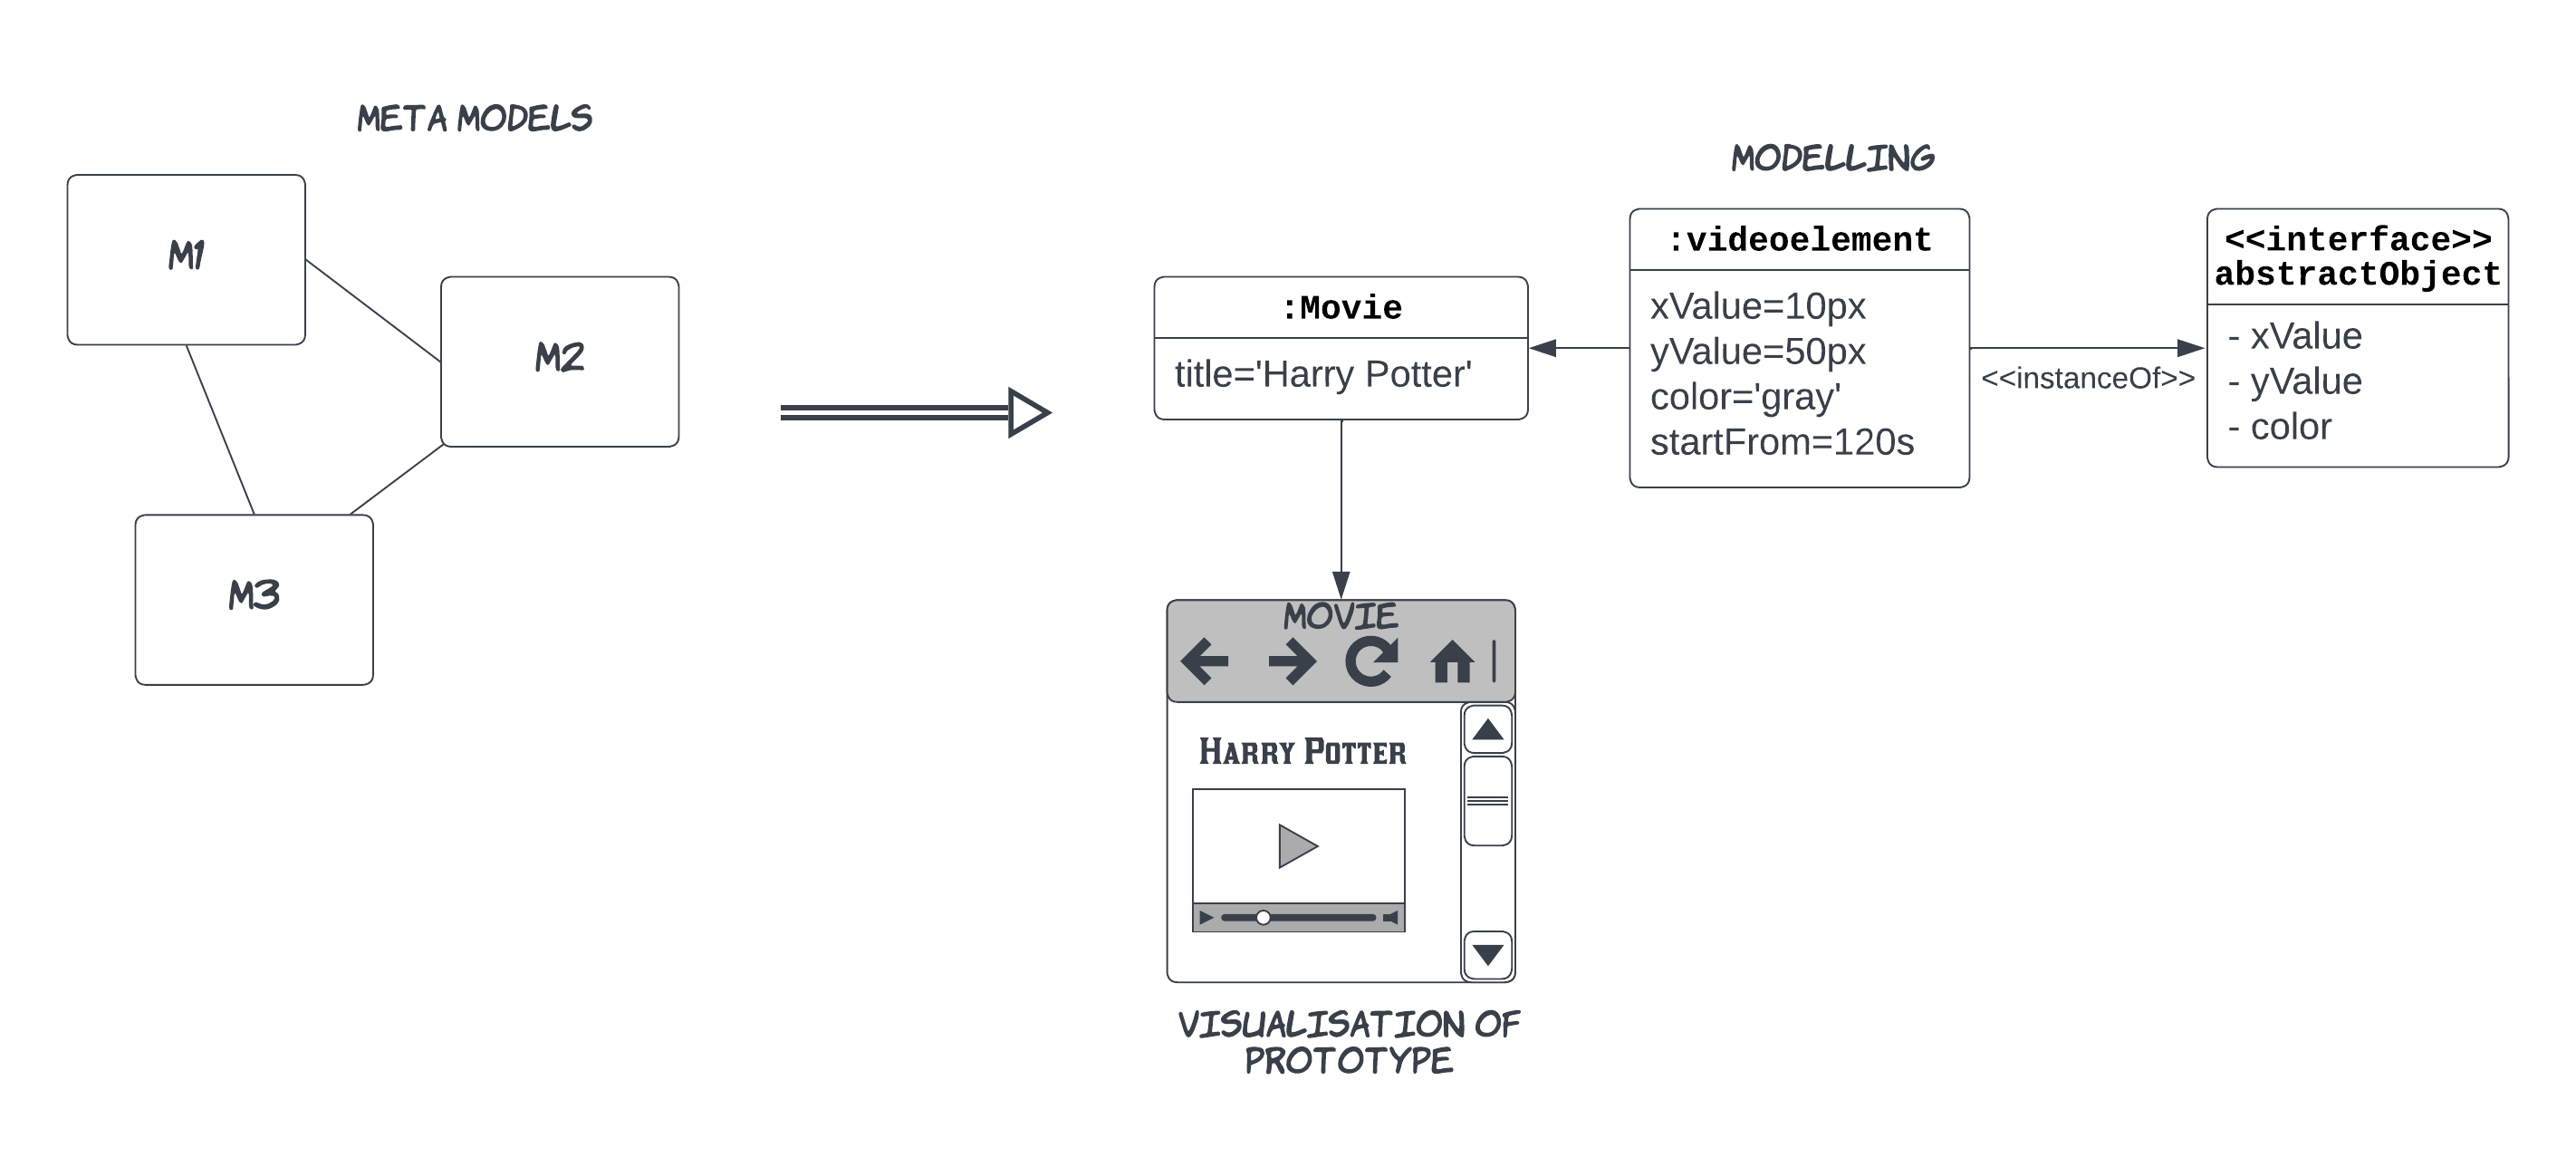
\includegraphics[width=1.05\textwidth]{images/solution-ideas/MetaModel.png}
	\caption{Example Modelling of Prototypes}
	\label{solutionideas:fig:metamodel}
\end{figure}

\paragraph{Prototype:} In the \texttt{Prototype Model}, we store information about the prototypes and all their components as independent parts.
This model stores all the different screens available in a software application and links them.
As per figure \ref{solutionideas:fig:metamodel}, the Modelling part shows the abstract and the concrete models required for prototyping the UI elements. 
(e.g., The ``abstractObject'' is an interface that is inherited by all the UI elements that are concrete elements ``videoelement'' of the containers or the screens ``Movie'').

\paragraph{Experiment:} In the \texttt{Experiment Model}, we store different properties of the UI elements along with the variant information. 
As per figure \ref{solutionideas:fig:metamodel} the ``videoelement'' under modeling contains attributes to store the position of the video viewer, which is a concrete element.
Similarly, it can store some extra properties of the ``videoelement'' that are different from the ``abstractObject''.
Moreover, the models should be able to accept measurements (e.g., \texttt{ClickRate} to measure the user clicks, \texttt{ViewTime} to measure the time spent by the user) to determine the best fit among the variants.
This way, we can create simple Experiments on the users (e.g., changing the position of the UI elements using the drag-and-drop feature).

\paragraph{Task:} In the \texttt{Task Model}, we store a sequence of activities that the user needs to perform and obtain feedback as measurements from the users for testing the software product.
This activity sequence is stored in the models and linked to the users.
The models should be able to accept the Measurements (like the Experiment models) to get feedback from the users (e.g., \texttt{ClickRate} and \texttt{ViewTime}). 

\begin{figure}[h]
	\centering
  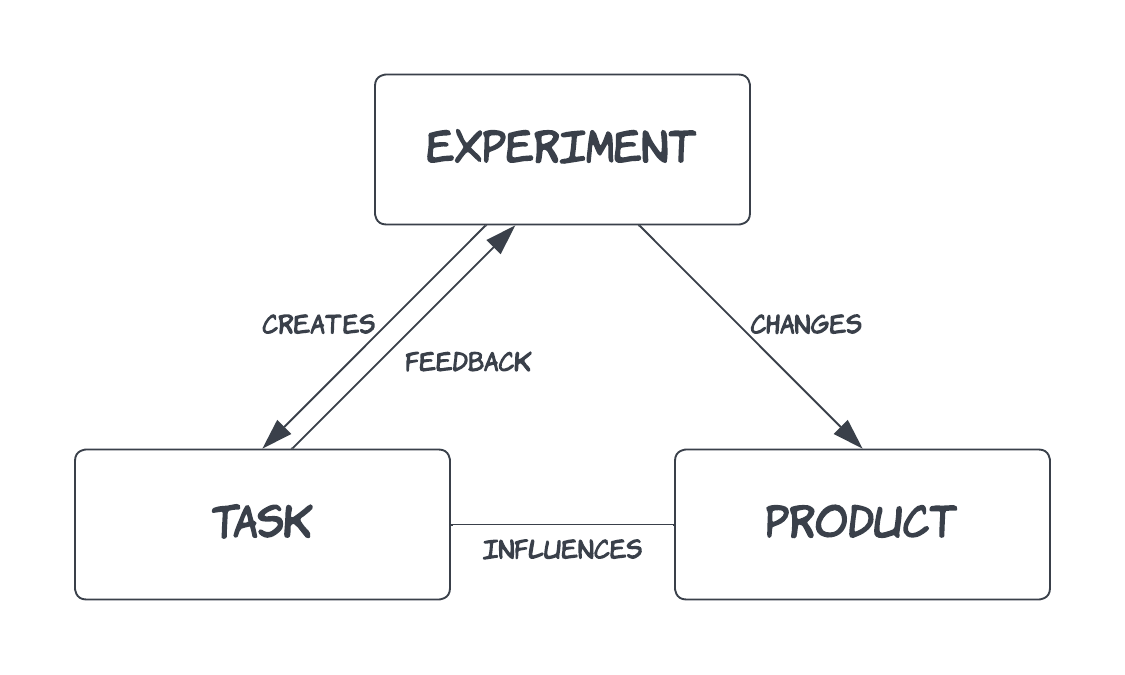
\includegraphics[width=0.7\textwidth]{images/solution-ideas/Triangle.png}
	\caption{Triangle of Experiment, Task, and Prototype}
	\label{solutionideas:fig:triangle}
\end{figure}
% E.g., from \texttt{Videostreamer app}: If the experiment is on a \texttt{Button} element, our model should have information about the position of the button, the style of the button (storing the color, font, etc.), the title of the button, etc. 
% All this information would be stored in the model as its properties or attributes.
% The Model also stores information of different variants of a particular application screen. (E.g., see figure \ref{solutionideas:fig:experimentingvariants} the Grid and the List View)
% E.g., from \texttt{Videostreamer app}: We would give a task to a user U1, saying ``Navigate to the movie M1'' and measure the number of steps/clicks and the time required for the user to perform this task.

We try to relate these models as depicted by the figure \ref{solutionideas:fig:triangle} in a triangle relationship.\\ 
\texttt{(1) Experiment-Task, (2) Experiment-Prototype, and (3) Task-Prototype} relationships.

\paragraph{Experiment-Task:} An experiment can create various tasks for the users and get some feedback in the form of data from the Task model. 

\paragraph{Experiment-Prototype:} From an experiment, it can be decided which is the best variant for the prototype and can thus modify and improve the prototype in an iteratively continuous process.

\paragraph{Task-Prototype:} A task should be created based on the current state of the product, and thus it creates a relationship between the task and the product.


\section{Measure}
The prototypes, experiments, and tasks are ready to be assigned to the users. 
So, in this section, we explain how they are allocated to the users (see section \ref{solutionideas:subsection:usertesting}) and collect feedback (see section \ref{solutionideas:subsection:measurements}) from them for improving the prototypes.

\subsection{Prototypes for User Testing}
\label{solutionideas:subsection:usertesting}

The product owners continuously investigate new features and product enhancement opportunities. 
The owners better understand their customers' experiences by creating that feedback loop with users. 
As a result, they need to conduct experiments.
In these experiments, the population (i.e., all users) is divided into small user groups, each receiving a unique variant. 
This type of setup is called the ``\texttt{Between-group}'' design experiment. 
As mentioned earlier, we also create tasks for the users allocating the tasks to the users performing experiments.  
As shown in figure \ref{solutionideas:fig:experimentingvariants}, the experiment model creates different variants for the prototype \texttt{View}: the \texttt{Grid view} (on the left) and the \texttt{List view} (on the right). 
These experiments are conducted on the users by dividing the users into groups and assigning one of the variants to a group. 
Then, the tasks are created for the specific experiment (e.g., Locate Movie M1). So, all the users with their experiment variant will try to complete the task.
The data are measured (explained in section \ref{solutionideas:subsection:measurements}), analysed (explained in section \ref{solutionideas:section:dataanalysis}), and finally, we find the best variant for the prototype.

\begin{figure}[ht]
	\centering
  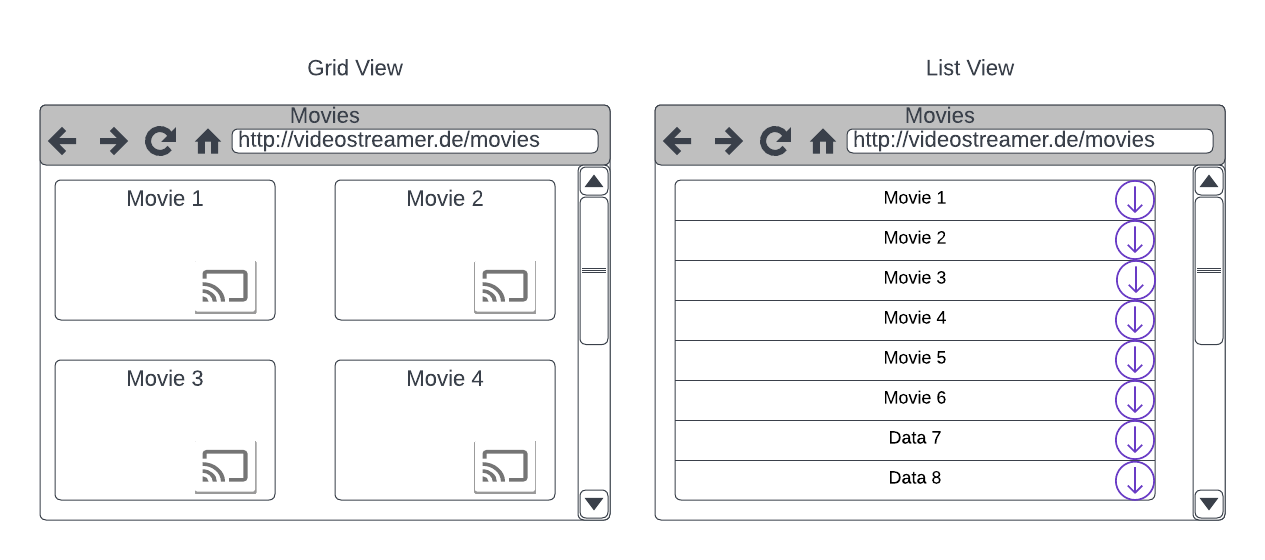
\includegraphics[width=1.0\textwidth]{images/solution-ideas/Experimentvariants.png}
	\caption{Example Experiment variants}
	\label{solutionideas:fig:experimentingvariants}
\end{figure}

\subsection{Measuring the Experiment and Task results}
\label{solutionideas:subsection:measurements}
To measure the experiment variants' performance, we add attributes to the models called ``Measurements''.
This attribute stores the voluntary (e.g., the number of clicks the user makes) and involuntary (e.g., the time required for the user to complete a task) user activities.
This attribute gets updated when the users perform the Task assigned to them by the \texttt{Task Model}.
(e.g., The task is to locate a movie for a registered user, so the user must log in, go to the movies page and search for the film, or scroll to find the film and click on the movie's title to play it.)
The UI variant (List or Grid View) assigned to the user plays a vital role in making this process smooth.
Therefore, measuring the Time or the Clicks required to reach the goal can be a critical factor in deciding the better variant.
After collecting the data from the experiment variants, we do an analyses (see section \ref{solutionideas:section:dataanalysis}) and improve prototype (see section \ref{solutionideas:subsection:improvingprototypes})

\section{Learn}
In this section, we do the analyses (see section \ref{solutionideas:section:dataanalysis}) from the data collected during the Experiments, get feedback on the better experiment's variant, and improve our prototype (see section \ref{solutionideas:subsection:improvingprototypes}).
\subsection{Analysis}
\label{solutionideas:section:dataanalysis}

In our solution, we focus on data-driven development. 
To determine the ``Winner'' among the variants of a product's component, we perform data analytics on the feedback data we receive from the \texttt{Task Model} and the \texttt{Experiment Model}.
We perform the \texttt{Quantitative} (presented in section \ref{solutionideas:paragraph:quantitative}), \texttt{Qualitative} (presented in section \ref{solutionideas:paragraph:qualitative}), and the \texttt{Task} (presented in section \ref{solutionideas:paragraph:taskanalysis}) analyses of the data.

% \begin{figure}[ht]
% 	\centering
%   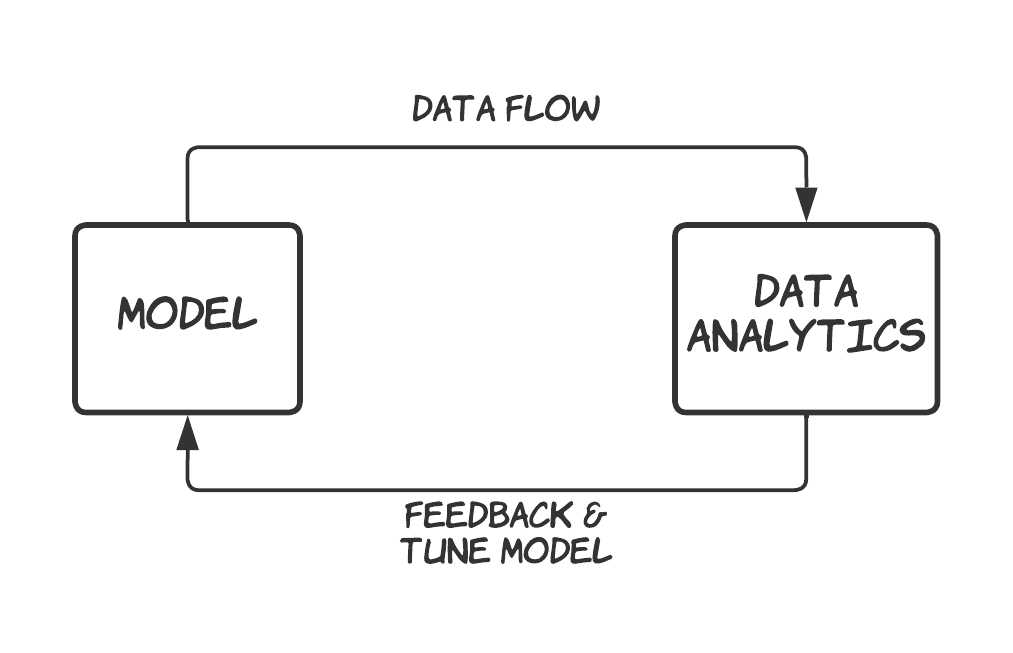
\includegraphics[width=0.5\textwidth]{images/solution-ideas/dd-development.png}
% 	\caption{Model-based \& Data Driven development}
% 	\label{solutionideas:fig:dddevelopment}
% \end{figure}

\paragraph{Quantitative Analysis:}
\label{solutionideas:paragraph:quantitative}
Quantitative analysis uses mathematical and statistical methods to determine the behavior of the data.
In quantitative research, various descriptive statistics methods like Means, Median, Variances, Standard Deviations, etc., are used to find some causal relationships in the data.
After collecting the data, the experimenting server can calculate the measurements' mean (assume the mean is specified in the experiment).
But, it isn't easy to generalize the results using means or descriptive statistical methods. 
Therefore, a significance test can be calculated to validate the probability of the event's occurrence, claim from the mean, and declare the winner variant.

\paragraph{Qualitative Analysis:}
\label{solutionideas:paragraph:qualitative}
To further improve, we need to perform qualitative analysis.
Qualitative analysis is used to determine the users' behavior and semantics.
Qualitative research data is usually unstructured, coming from open-ended surveys, interviews, etc. 
Our goal is to turn the unstructured data into a detailed description of the critical aspects of the problem.
In our solution, we propose to perform a qualitative analysis of the data by asking some open-ended questions to the users
(e.g., questions like ``What do you think about the Look and feel of the software application?'', ``Are the items on the page easily locatable?'', etc.).
The users' responses can be studied using some tools using the inductive or deductive coding technique. 
% If we select the inductive coding approach, we will scrutinize the reactions and those which are similar and group them. 
% These groups will be coded into labels, and we will formalize and analyze the categories. 
% To understand the process better, see figure \ref{solutionideas:fig:qualitative}. 
So, in the end, we get feedback from this process on which variants are better for the users. 
This information is forwarded to the models for modifying the prototypes.

% \begin{figure}[ht]
% 	\centering
%   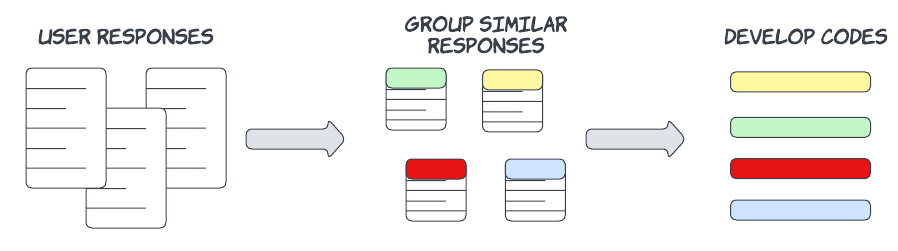
\includegraphics[width=1\textwidth]{images/solution-ideas/qualitative.png}
% 	\caption{Qualitative analysis using inductive coding}
% 	\label{solutionideas:fig:qualitative}
% \end{figure}

\paragraph{Task analysis:}
\label{solutionideas:paragraph:taskanalysis}
We also receive the data from the \texttt{Task Model}. 
Its data can be used to calculate the efficiency of the variant. 
A task model contains measurements for getting feedback from the users. 
E.g., If the task is to locate a particular movie, we can calculate the number of clicks and time required as measurements for the users to reach their destination.
This testing type is called ``\texttt{Supervised testing}'' \cite{article:dataanalysis:supervisedtest}.
So, we observe the users, and they know the result (i.e., the movie they need to locate). 
This process gives us more accurate feedback on which variant performs better, and we can then update the prototype as per our triangle relationship (see fig \ref{solutionideas:fig:triangle}).

\subsection{Improving the Prototype}
\label{solutionideas:subsection:improvingprototypes}
As per the LEAN development process, this is the final step in the cycle (see figure \ref{intro:fig:lean}) of that iteration.
After analyzing the data from experiments, we can conclusively claim with statistical evidence the ``winner'' variant of a component.
This helps us to tune our model by adding a ``default'' attribute and setting its value to be of the ``winner'' variant.
So, in the next iteration cycle, for the component, the ``winner'' variant is selected as default for future experiments.
After modifying our model, we can visualize the changes by observing the UI Prototypes.
E.g., In the \texttt{View} component of the \texttt{Videostreamer} app, the \texttt{GridView} is determined to be more usable as per the experiment and is declared the winner. 
Therefore, in the next iteration, the \texttt{default} attribute in the \texttt{View} component will be set to \texttt{GridView} for the following experiments.
\chapter{Structure of the Thesis} \label{sec:structure}

We plan to have our final thesis structure approximately in the following format: 

\begin{enumerate}
	\item Introduction
	\begin{itemize}
		\item Motivation
		\item Problem Statement
		\item Research Approach
		\item Solution Approach
	\end{itemize}
	\item Related Work
	\begin{itemize}
		\item State-of-the-art research
		\item Defining requirements / Research Questions
		\item Comparison
	\end{itemize}
	\item Background/Foundation (Here, explain in detail the topics needed for developing a basis for the thesis. Some of the topics include:)
	\begin{itemize}
		\item Continuous Experimentation
		\item Low code / No Code techniques
		\item Model-based Software engineering
		\item Data-driven Engineering
		\item A/B Testing, etc. 
	\end{itemize}
	\item Design (As per LEAN development technique)
	\begin{itemize}
		\item Build
		\item Measure
		\item Learn
	\end{itemize}
	\item Implementation
	\begin{itemize}
		\item Architecture
		\item Implementation of Prototypes, Experiments and Tasks
		\item Execution of POC
	\end{itemize}
	\item Evaluation
	\begin{itemize}
		\item Discussions for opportunities and Risks
		\item Limitations
	\end{itemize}
	\item Conclusion and Future Work
\end{enumerate}

These chapters are used for creating the Work Packages and a timeline for the thesis (explained in Chapter \ref{chap:wps}).
\chapter{Work Packages and Timeline}
\label{chap:wps}
In this section, we define the work packages, and timeline to fulfill the defined tasks in the next months.

\section{Work Packages}
We divide our thesis into Work packages (WP) or Tasks.
This can be used to track the progress of the thesis and get feedback.

\paragraph{WP1 (Introduction):} In this package, we would like to start by introducing the topic, identifying the problems by defining the problem statement, and finally, defining our research and solution approach.
\begin{enumerate}
    \item Motivation
    \item Problem Statement
    \item Research and Solution Approach
\end{enumerate}

\paragraph{WP2 (Related Work):} Here, we would like to find some State-of-the-art research and compare them with the research questions or the requirements that we define for the thesis.
\begin{enumerate}
    \item State-of-the-art research
    \item Defining requirements / Research Questions
    \item Comparison
\end{enumerate}

\paragraph{WP3 (Foundation):} In this package, we would like to define some terminologies according to the research (e.g., Continous Experimentation, Low-Code, etc.)

\paragraph{WP4 (Design):} Here, we would like to design our thesis as per the LEAN development cycle, containing Build, Measure and Learn phases.
\begin{enumerate}
    \item Build
    \item Measure
    \item Learn
\end{enumerate}

\paragraph{WP5 (Implementation):} In this package, we would like to implement the prototypes by developing the meta-models, defining the architectures, and coding them for visualization of the prototypes.
We would also conduct experiments on the users and measure and learn from their feedback.
\begin{enumerate}
    \item Architecture
    \item Creating meta models and concrete models for database 
    \item Visualization of the Prototypes 
\end{enumerate}

\paragraph{WP6 (Testing the prototypes):} In this package, we would test our prototypes by creating the experiments and the tasks for the users and measuring feedback from them.
\begin{enumerate}
    \item Deployment on Server using docker\footnote{Docker: \url{https://www.docker.com/}}
    \item Create and assign experiments, and tasks to the users 
    \item Analyze the measurements
\end{enumerate}

\paragraph{WP7 (Evaluation):} Every research has Opportunities, Risks, and Limitations. In this WP, we would be discussing them.
\begin{enumerate}
    \item Opportunities
    \item Risks
    \item Limitations
\end{enumerate}

\paragraph{WP8 (Conclusion):} Here, we conclude the thesis and write the scope for future work.
\begin{enumerate}
    \item Conclusion
    \item Future work
\end{enumerate}

\section{GanttChart for Timeline}
% \subsection{GanttChart Simple}
% \begin{ganttchart}
% 	[today=0, %"TODAY" vertical line
% 	]{1}{26}
% 	\gantttitle[title label node/.append style={below left=7pt and -3pt}]{WEEKS:\quad1}{1}
% 	\gantttitlelist{2,...,26}{1} \\
% 	\ganttgroup[progress=0]{WP1}{1}{4} \\
% 	\ganttgroup[progress=0]{WP2}{5}{6} \\
% 	\ganttgroup[progress=0]{WP3}{7}{16} \\
% 	\ganttgroup[progress=0]{WP4}{16}{23} \\
% 	\ganttgroup[progress=0]{WP5}{21}{26}\\
	
% 	\ganttmilestone{Milestone 1}{4}\\
% 	\ganttmilestone{Milestone 2}{8}\\
% 	\ganttmilestone{Milestone 3}{12}\\
% 	\ganttmilestone{Milestone 4}{16}\\
% 	\ganttmilestone{Milestone 5}{20}
% \end{ganttchart}


% \subsection{GanttChart Detailed}
This section gives a rough estimation of the time required for the WPs execution.
We divide the entire time period of the thesis into 26 weeks, with the first four weeks dedicated to the Proposal or the Exposée.

\begin{ganttchart}
	[today=0, %"TODAY" vertical line
	vgrid,
    hgrid,
	progress label text={},
	]{1}{26}
	\gantttitle[title label node/.append style={below left=7pt and -3pt}]{WEEKS:\quad1}{1}
	\gantttitlelist{2,...,26}{1} \\
	\ganttgroup[progress=0]{WP1}{1}{3} \\
	\ganttgroup[progress=0]{WP2}{5}{6} \\
	\ganttgroup[progress=0]{WP3}{2}{4} \\
	\ganttgroup[progress=0]{WP4}{7}{9} \\
		\ganttbar[progress=0]{\textbf{WP 4.1}}{7}{7} \\
		\ganttbar[progress=0]{\textbf{WP 4.2}}{8}{8}\\
		\ganttbar[progress=0]{\textbf{WP 4.3}}{9}{9}\\
	\ganttgroup[progress=0]{WP5}{8}{11}\\
		\ganttbar[progress=0]{\textbf{WP 5.1}}{8}{9}\\
		\ganttbar[progress=0]{\textbf{WP 5.2}}{9}{11}\\
		\ganttbar[progress=0]{\textbf{WP 5.3}}{10}{11}\\
	\ganttgroup[progress=0]{WP6}{11}{20}\\
		\ganttbar[progress=0]{\textbf{WP 6.1}}{11}{16}\\
		\ganttbar[progress=0]{\textbf{WP 6.2}}{14}{15}\\
		\ganttbar[progress=0]{\textbf{WP 6.3}}{13}{20}\\
	\ganttgroup[progress=0]{WP7}{19}{23}\\
	\ganttbar[progress=0]{\textbf{WP 7.1}}{19}{21}\\
	\ganttbar[progress=0]{\textbf{WP 7.2}}{21}{23}\\
	\ganttbar[progress=0]{\textbf{WP 7.3}}{22}{23}\\
	\ganttgroup[progress=0]{WP8}{22}{24}\\
	% \ganttgroup[progress=0]{Buffer}{25}{26}\\
	% \ganttmilestone{Milestone 1}{4}\\
	% \ganttmilestone{Milestone 2}{8}\\
	% \ganttmilestone{Milestone 3}{12}\\
	% \ganttmilestone{Milestone 4}{16}\\
	% \ganttmilestone{Milestone 5}{20}
\end{ganttchart}


\pagestyle{scrplain} % turn off headers and footers

\KOMAoptions{open=any} % Plaziert Kapitel auch auf linken Seiten

%% generate bibliography with bibtex, the bibfile here is "paper.bib"
\flushbottom
\bibliographystyle{plainnat}
\bibliography{literature/literature,rfcbib/data/rfc.bib,cryptobib/crypto.bib}

\end{document} 
